\chapter{Introduction}

\section{Background}
Ferromagnetic materials (FM) known to humanity for more than 2000 years. It's been a long time since the first samples of a mineral known as lodestone (\ce{Fe_3O_4}) amazed our ancestors by its unique properties. Since then, this class of materials was thoroughly analyzed and described by many generations of bright scientists. But yet even in the 21st century, we still have many questions to answer to fully understand this mysterious phenomenon. 

The wide usage of FM materials in industrial applications started in the late 19th century when carbon steels were replaced with Alnico alloys.  Futher the discovery of the large magnetocrystalline anisotropy in the second part of the 20th century lead to the revolutionary introduction of rare-earth magnets. First produced samples of \ce{Sm_5Gd} reported in 1960 lead to an industrial breakthrough and further rapid development in this field.  From this moment, the remarkable increase in the energy product of magnetic materials was accompanied by the tremendous decrease in their volume, providing the same amount of magnetic energy as it is illustrated in figure~\ref{fig:history}.  Progress in this direction ends up with the discovery of the strongest and most usable till now Nb-Fe-B composition \cite{Gutfleisch2010}. 

Nowadays, FM are actively used not only in the design of complex technical devices such as engines, turbines, and generators but also as an irreplaceable part of widely used mass-market consumer products. Mobile phones, laptops, hard drives, audio devices, and an endless number of other applications have made this class of materials one of the most sought-after in the present times. As a result, the need for strong and cheap magnets has increased hundreds of times in just the last few decades with a special interest in rare-earth (REEs) magnets possessing excellent properties at room temperature within a relatively low price per energy-density unit.
But at this point, the modern world faced quite a risky situation. Thus, according to the recent data of the World Trade Organization, more than 95\% of REEs mining concentrated in China. This monopoly has led to a rapid rise in prices for REEs over the past few years and is undoubtedly unsatisfactory for countries with a high demand for these materials. Moreover, the strong concentration of such a critical resource in one place in the event of unforeseen circumstances (such as COVID-19) can cause a complete interruption in supplies and multibillion money losses for manufacturers around the globe.

\begin{figure}[H]
	\centering
	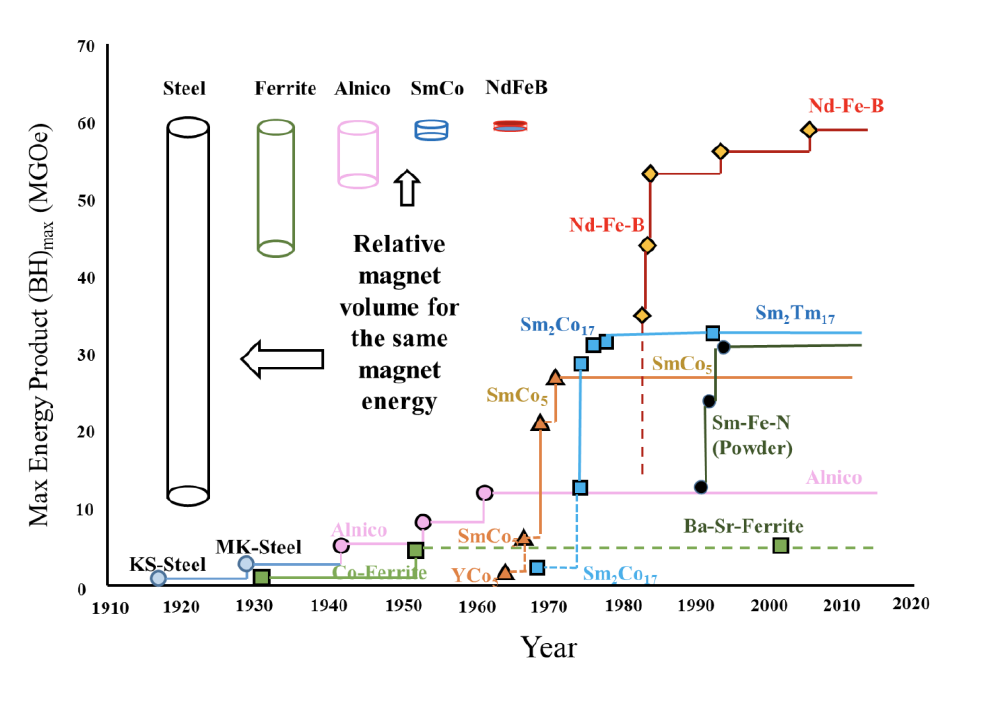
\includegraphics{fig/review/history.png}
	\caption[Development in energy product of permanent magnetic materials]{Development in energy product of permanent magnetic materials.}
	\label{fig:history}
\end{figure}

The possessed situation lead to a great interest of science and industry in discovering new ferromagnetic materials. Nevertheless, despite several attempts to computationally predict new structures made in the last 25 years, this problem remains unsolved. One reason for it is a limitation of modern algorithms, which allows to exact only elementary properties like stability and magnetic moment, staying absolutely blind to FM critical temperature. As a consequence, a huge amount of computational and experimental efforts results in materials with low technological potential due to unsatisfying values of Curie temperature. 


\cleardoublepage
\section{Aim and Goals}


Based on a brief introduction, the ultimate goal of this study is to search for new technologically promising magnetic compositions. Considering the capabilities of modern evolutionary algorithms that allow identifying stable structures with a high magnetic moment, the problem of automated determination of the critical magnetic temperature (Curie point) remains unsolved. To solve the indicated problem and empower the end-user with a straightforward methodology for its calculation, the following research objectives are identified:


\begin{enumerate}
\item Development and implementation of the critical magnetic temperature calculation methodology based on DFT approaches followed by Monte Carlo simulations.
\item Training of several classical ML models to solve a regression problem of critical temperature estimation based on the available experimental data.
\item Testing of the developed methods on compositions with known experimental and theoretical values of Curie temperature.
\item Computational search for new compositions with high magnetic properties using evolutionary algorithm USPEX \cite{Oganov_2006, Oganov_2011,  Oganov_2013}.
\item Benchmarking of the newly find structures concerning their critical temperature to
determine the most promising from the technological viewpoint.
\end{enumerate}

\section{Outline}

Chapter 1 contains the current section with a problem background and formulation of the project objectives. Chapter 2 contains a general overview of the ferromagnetic materials properties and theoretical models used for this study. Chapter 3 describes the methodology used in this work, namely the construction of several machine learning (ML) models over available experimental data and calculations based on density function theory (DFT) followed by Monte-Carlo (MC) simulations. Chapter 4 is dedicated to the discussion of the results obtained by both methods. Finally, chapter 5 summarizes the research outcome and outlines possible future studies.



